\PassOptionsToPackage{colorlinks,linkcolor={blue},citecolor={blue},urlcolor={blue},breaklinks=true,final}{hyperref}
\PassOptionsToPackage{dvipsnames}{xcolor}
\documentclass[xcolor={dvipsnames,svgnames},aspectratio=169]{beamer}

\usepackage{fontawesome5}
\usepackage{booktabs} % For better table formatting
\usepackage{listings}

\lstset{
  tabsize = 4, %% set tab space width
  showstringspaces = false, %% prevent space marking in strings, string is defined as the text that is generally printed directly to the console
  numbers = left, %% display line numbers on the left
  commentstyle = \color{purple!60}, %% set comment color
  keywordstyle = \color{blue}, %% set keyword color
  stringstyle = \color{red}, %% set string color
  rulecolor = \color{black}, %% set frame color to avoid being affected by text color
  basicstyle = \small \ttfamily , %% set listing font and size
  breaklines = true, %% enable line breaking
  numberstyle = \tiny,
}

\title{Concurrent Programming}
\subtitle{Week 10 (Lecture 2)}
\author{Stelios Tsampas}
\institute{
  \faEnvelope \; stelios@imada.sdu.dk
  \qquad
  \faGlobe \;
  \href{https://www.steliostsampas.com}{https://www.steliostsampas.com}
  \\\\\
  \faGithub \; stelios-tau/cp-2025
  \qquad\;\;
    \faDiscord \; cp-2025
}
\date{February 17, 2025}

\titlegraphic{
\includegraphics[height=0.6cm,keepaspectratio]{../media/sdu-black.eps}}

\usetheme[block=fill]{metropolis}


%\usepackage{pres-common}
\usepackage{textpos}
\usepackage{centernot}

% \newcommand{\Goesv}[3]{\ensuremath{#1 \xRightarrow{~#3~} #2}}
% \newcommand{\goesv}[3]{\ensuremath{#1 \xrightarrow{~#3~} #2}}

% \usepackage{etex}
% \usepackage{semantic}

\usepackage[utf8]{inputenc}
\usepackage[english]{babel}
\usepackage{tikz}
\usepackage{hyperref}

\usetikzlibrary{arrows,shapes,matrix}
\usetikzlibrary{backgrounds}
\usetikzlibrary{positioning}
\usetikzlibrary{automata}
\usetikzlibrary{mindmap}
\usetikzlibrary{shapes.callouts}
\usetikzlibrary{decorations.text}
\usetikzlibrary{tikzmark}
\usetikzlibrary{calc}
\usetikzlibrary{overlay-beamer-styles}

\tikzset{onslide/.code args={<#1>#2}{%
    \only<#1>{\pgfkeysalso{#2}} % \pgfkeysalso doesn't change the path
  }}

\setbeamercolor{mygray}{bg=Gray!20}

\tikzset{temporal/.code args={<#1>#2#3#4}{%
    \temporal<#1>{\pgfkeysalso{#2}}{\pgfkeysalso{#3}}{\pgfkeysalso{#4}} % \pgfkeysalso doesn't change the path
  }}

\tikzstyle{highlight}=[fill=green!50]
\tikzstyle{hgreen}=[fill=green!20]
\tikzstyle{hred}=[fill=red!50]
\tikzstyle{hblue}=[fill=blue!50]
\tikzstyle{hgray}=[fill=gray!50]

\addtobeamertemplate{frametitle}{}{%
\begin{textblock*}{100mm}(\textwidth-2cm,-0.86cm)

\includegraphics[height=0.6cm,keepaspectratio]{../media/sdu-white.eps}
\end{textblock*}}

%\usepackage{tikz-cd}
% \usepackage{wasysym}
% \usepackage{color}
% \usepackage[matrix,arrow]{xy}
% \xyoption{all}
% \SelectTips{cm}{}
% % \usepackage{cite}
% \usepackage{amsthm}
% \usepackage{amsmath}
% \usepackage{bbold}
% % \usepackage[bbgreekl]{mathbbol}
% \usepackage{amssymb}
% \usepackage{pifont}
% \usepackage{mathtools}
% \usepackage{amsbsy}
% % \usepackage{paralist}
% \usepackage{shadethm}
% % \usepackage{fancyhdr}
% \usepackage{stmaryrd}
% \usepackage{wasysym}
% \usepackage{graphicx}
% \usepackage{tabularx}
% \usepackage{dsfont}
% \usepackage{ulem}




%\bibliography{mainBiblio}

%\includeonlyframes{current}
\begin{document}

\frame{\titlepage}

\def\firstcircle{(0,0) circle (2cm)}
\def\secondcircle{(1.4,1.4) circle (2cm)}
\def\thirdcircle{(0:2.4) circle (2cm)}

\begin{frame}{Outline}
  \tableofcontents
\end{frame}

\section{Previously, on Week 8}

\begin{frame}[fragile]
  \frametitle{Examples of Concurrency}

  Picture a chef (or more than one) cooking multiple dishes at the same time:

  \begin{itemize}
  \item[\faBook]<1-> The chef prepares multiple meals at once by switching tasks.
  \item[\faBook]<2-> They might chop vegetables, then stir a sauce, then check the oven.
  \item[\faBook]<3-> The dishes are interleaved but not truly parallel.
  \end{itemize}
\end{frame}

\begin{frame}[fragile]
  \frametitle{Case 1: one chef}

  \begin{center}
    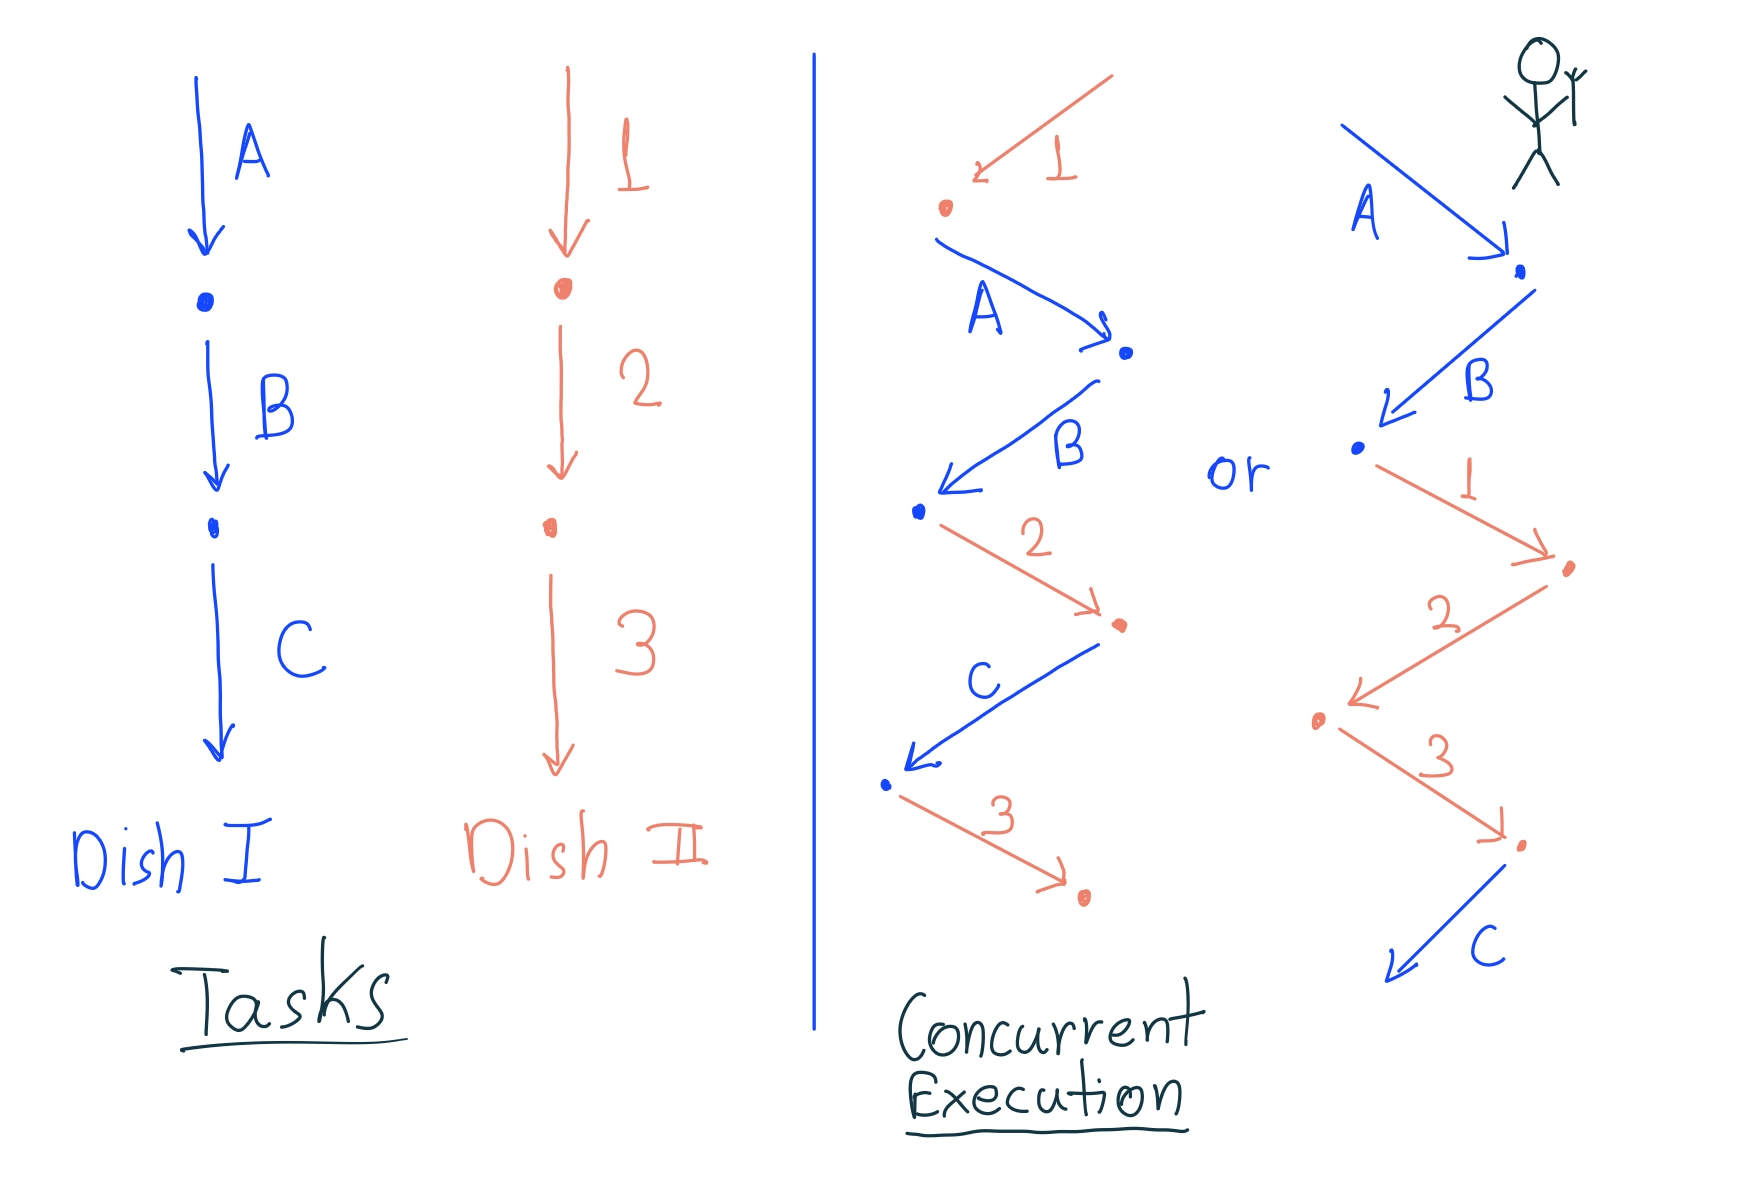
\includegraphics[width=11cm,keepaspectratio]{../media/lecture1-chef.png}
  \end{center}

  \onslide<2->{
    \begin{tikzpicture}[overlay, remember picture]
      \node[xshift=3cm,yshift=5cm,starburst,starburst points=30,
      align=center,fill=yellow, opacity=1,draw=red, line width=2pt]
      {\textbf{Nondeterministic \faSkullCrossbones}};
    \end{tikzpicture}}

\end{frame}

% \begin{frame}[fragile]
%   \frametitle{Case 1: one chef}

%   \large{
%   \begin{itemize}
%   \item[\faBook]<1-> You don't need more than one chef/CPU cores/threads to have
%     concurrent execution.
%   \item[\faBook]<1-> \textbf{Task switching}/\textbf{interleaving} are the hallmarks of
%     concurrency.
%   \end{itemize}}
% \end{frame}

\begin{frame}[fragile]
  \frametitle{Degenerate (non-)example, sequential execution}

  \begin{center}
    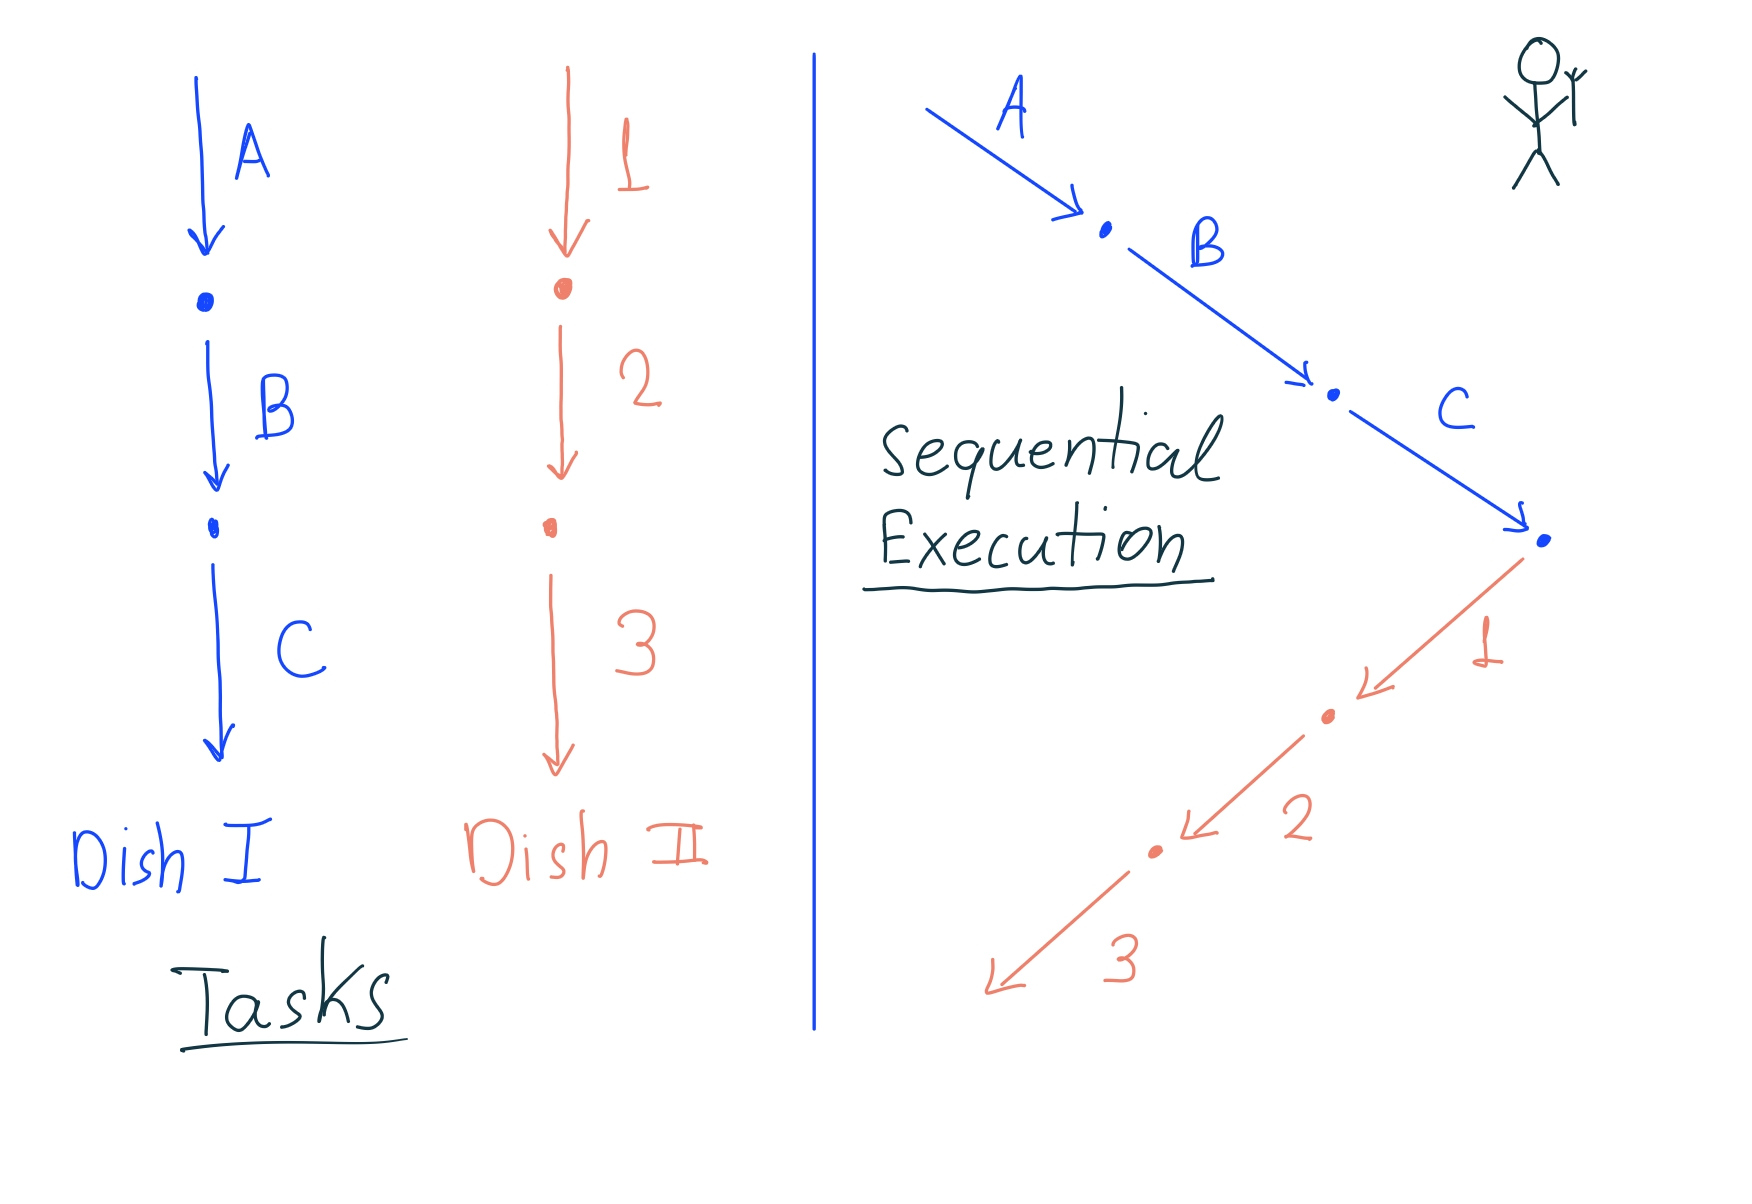
\includegraphics[width=11cm,keepaspectratio]{../media/lecture1-seq.png}
  \end{center}

  \onslide<2->{
    \begin{tikzpicture}[overlay, remember picture]
      \node[xshift=3cm,yshift=5cm,ellipse,
      align=center,fill=green!20, opacity=1,draw=black, line width=0.4pt]
      {\textbf{Predictable \faCheck}};
    \end{tikzpicture}}

\end{frame}

% \begin{frame}[fragile]
%   \frametitle{Degenerate (non-)example, sequential execution}

%   \large{
%     \begin{itemize}
%     \item[\faBook]<1-> In sequential execution, tasks are \emph{sequenced},
%       their execution will not be interrupted.
%     \item[\faBook]<2-> Simple and predictable, the kind of programming you have
%       been doing so far.
%     \end{itemize}}

% \end{frame}


\begin{frame}[fragile]
  \frametitle{Case 2: two chefs}

  \begin{center}
    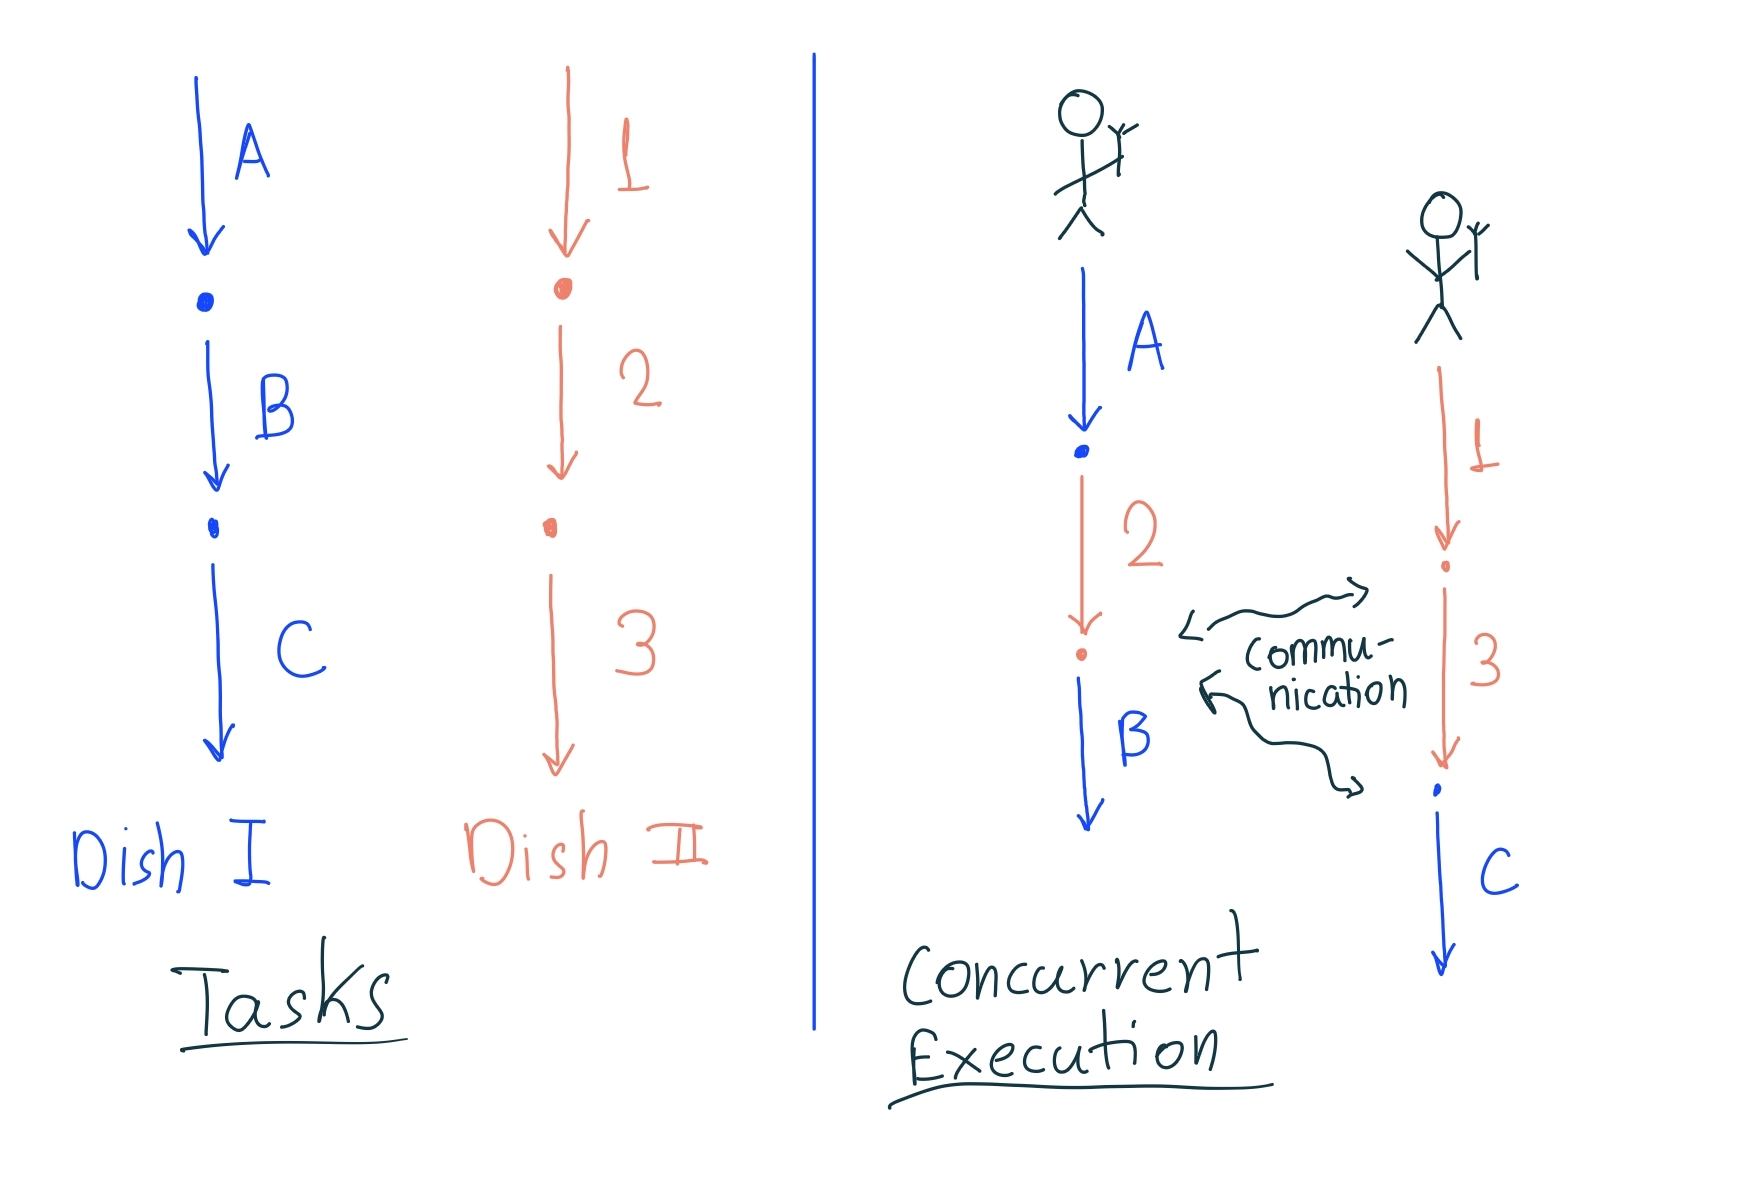
\includegraphics[width=11cm,keepaspectratio]{../media/lecture1-twochefs.png}
  \end{center}

  \onslide<2->{
    \begin{tikzpicture}[overlay, remember picture]
      \node[xshift=3cm,yshift=5cm,starburst,starburst points=30,
      align=center,fill=yellow, opacity=1,draw=red, line width=2pt]
      {\textbf{Nondeterministic \faSkullCrossbones}};
    \end{tikzpicture}}
\end{frame}

% \begin{frame}[fragile]
%   \frametitle{Case 2: two chefs}

%   \large{
%     \begin{itemize}
%     \item[\faBook]<1-> This time there are actually distinct chefs/\textbf{threads} of
%       execution taking place.
%     \item[\faBook]<2-> They might be sharing resources (i.e. using the same
%       equipment, food), so extra care needs to be taken, especially because the
%       interleaving is \textbf{non-deterministic}.
%     \item[\faBook]<3-> Remember that these \textbf{threads} are abstractions, it
%       is not necessary that, underneath the surface, their a multi-core CPU
%       executing each thread.
%     \end{itemize}}
% \end{frame}

\begin{frame}[fragile]
  \frametitle{Degenerate (non-)example 2, parallelism}

  \begin{center}
    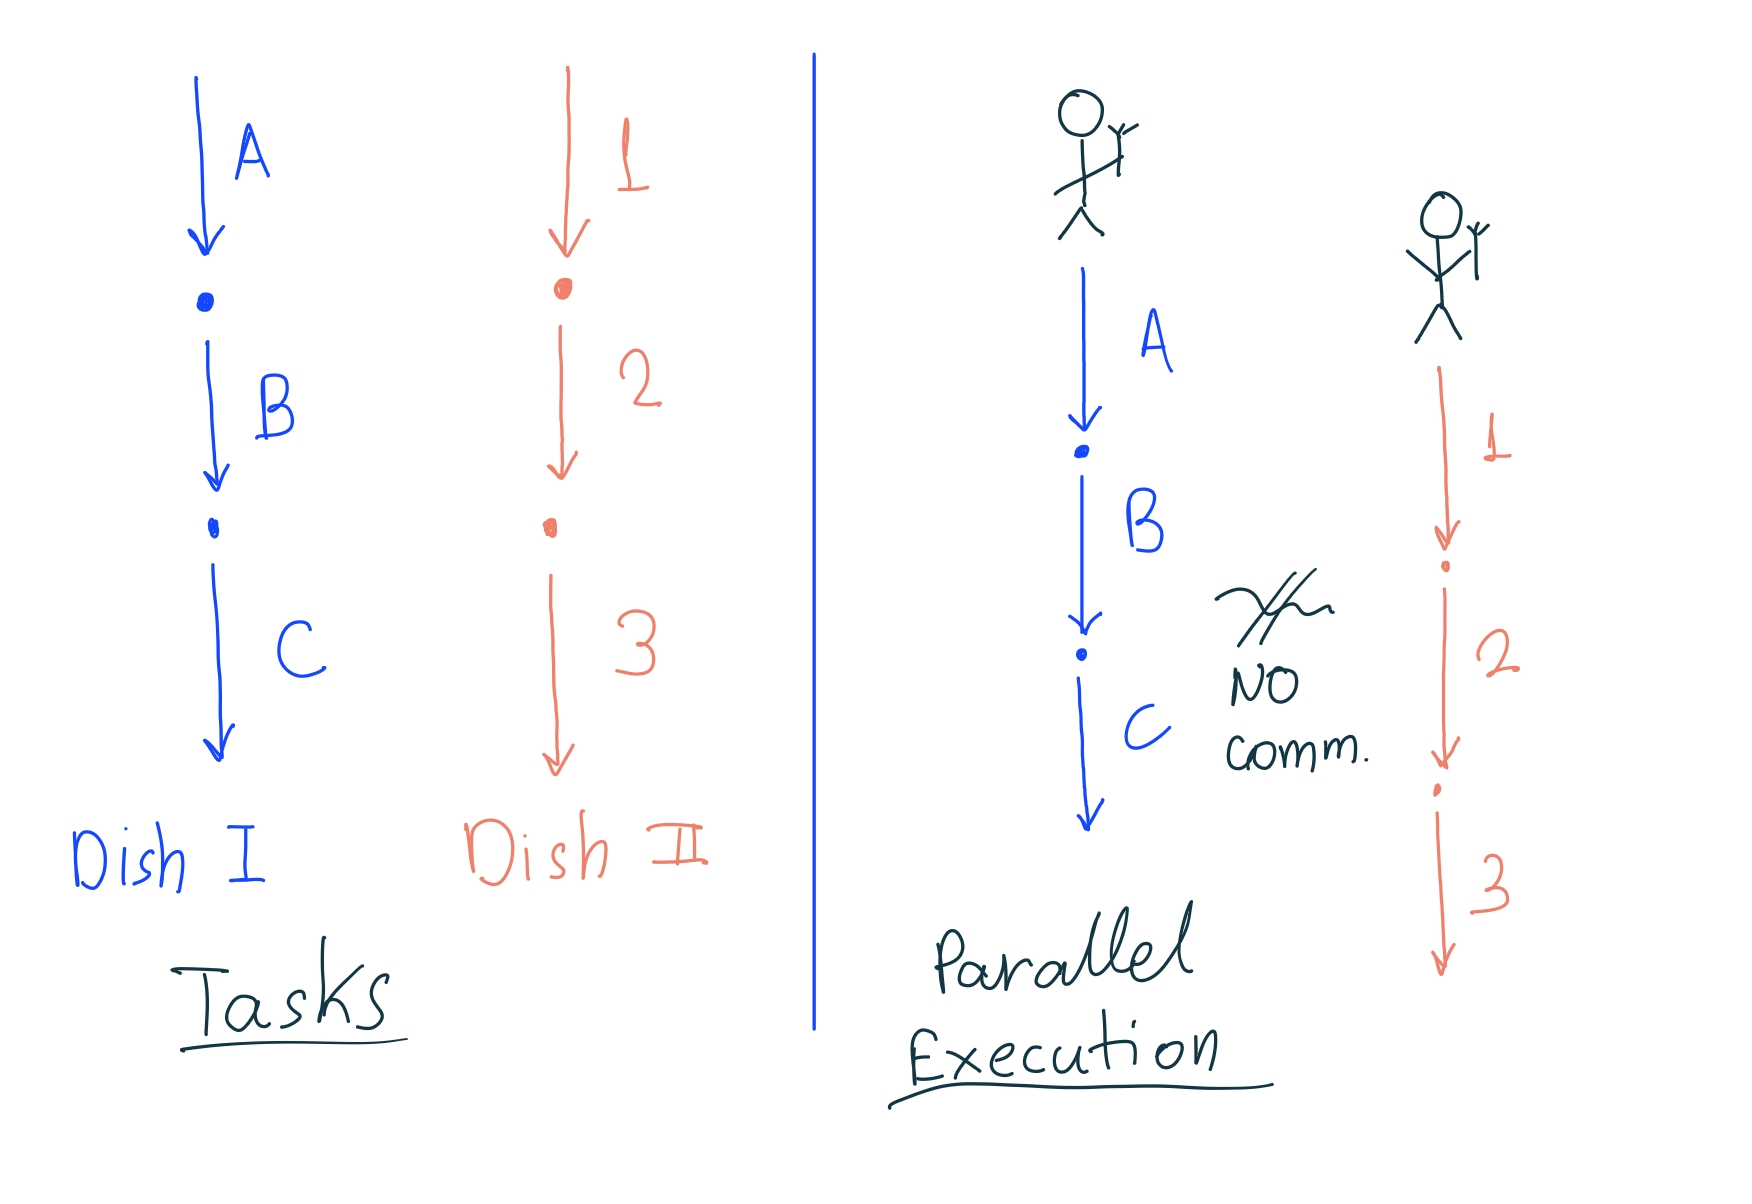
\includegraphics[width=11cm,keepaspectratio]{../media/lecture1-para.png}
  \end{center}

  \onslide<2->{
    \begin{tikzpicture}[overlay, remember picture]
      \node[xshift=3cm,yshift=5cm,ellipse,
      align=center,fill=green!20, opacity=1,draw=black, line width=0.4pt]
      {\textbf{Predictable \faCheck}};
    \end{tikzpicture}}
\end{frame}

% \begin{frame}[fragile]
%   \frametitle{Degenerate (non-)example 2, parallelism}

%   \large{
%     \begin{itemize}
%     \item[\faBook]<1-> Again, there are two chefs/\textbf{threads} of
%       execution taking place.
%     \item[\faBook]<1-> However, their tasks are distinct, and there is no
%       communication between the two.
%     \item[\faBook]<1-> This is \textbf{parallel programming}, a different topic
%       that is about the developing algorithms that make use of
%       multiple CPU units.
%     \item[\faBook]<2-> \textbf{Not} quite the topic of this class,
%       although the programming techniques involved may overlap.
%     \end{itemize}}

% \end{frame}

% \begin{frame}{Key Differences: Concurrency vs. Parallelism}
%   \vspace{-0.4cm}
% \begin{table}[]
%     \centering
%     \begin{tabular}{l|l|l}
%         \toprule
%       \textbf{Feature}
%       & \textbf{Concurrency}
%       & \textbf{Parallelism} \\
%         \midrule
%       \textbf{Definition}
%       & Interleaved execution
%       & True simultaneous execution\\
%         \midrule
%       \textbf{Execution}
%       & Task switching, may be single-core
%       & Requires multiple cores \\
%         \midrule
%       \textbf{Use Case}
%       & Responsiveness (UI, servers)
%       & Performance (big data, heavy comp.) \\
%         \midrule
%       \textbf{Hardware}
%       & Can work on single-core
%       & Requires multi-core CPU \\
%         \midrule
%       \textbf{Example}
%       & Multi-threading with task switching
%       & Multi-threading with multiple cores \\
%         \midrule
%       \textbf{Java}
%       & \texttt{Thread}, \texttt{ExecutorService}
%       & \texttt{ForkJoinPool}, \texttt{parallelStream()} \\
%       \midrule
%       \textbf{Resources}
%       & Shared resources, synchronization
%       & Little to no sharing and communication\\
%       \midrule
%       \textbf{Effect}
%       & Non-deterministic
%       & (Largely) deterministic\\
%         \bottomrule
%     \end{tabular}
%   \end{table}
%   \onslide<3->{
%     \begin{tikzpicture}[overlay, remember picture]
%       \node[xshift=4cm,yshift=3cm,starburst,starburst points=25,
%       align=center,fill=yellow, opacity=1,draw=red, line width=2pt]
%       {\large{\textbf{Complete chaos!}}};
%     \end{tikzpicture}
%     \begin{tikzpicture}[overlay, remember picture]
%       \node[xshift=11cm,yshift=3cm,ellipse,
%       align=center,fill=green!20, opacity=1,draw=black, line width=0.4pt]
%       {\large{\textbf{Predictable \faCheck}}};
%     \end{tikzpicture}}
% \end{frame}

\begin{frame}[fragile]
  \frametitle{What this is all about}

  \large{A large amount of this class is about managing the \textbf{sharing} of resources
  and generally the \textbf{communication} and \textbf{coordination} of these
  \textbf{threads} of execution. \uncover<2->{Yes, the term \emph{threads} is
    the technically correct term.}}
\end{frame}

\begin{frame}[fragile]
  \frametitle{Threads}

  \begin{itemize}
  \item[\faBook] The main abstraction that is involved in concurrency.
  \item[\faBook] A thread represents a lightweight, independent unit of
    execution.
  \item[\faBook] Threads are present at multiple levels of the
    software stack:
    \begin{itemize}
    \item[\faLinux] Operating system level, i.e. user and kernel threads.
    \item[\faCode] At the level of programming languages, Java threads, pthreads
      in C...
    \end{itemize}
  \item[\faBook] There can be many active threads active at the same time, i.e.
    \emph{concurrently}.
  \item[\faExclamation]<2-> ... but they do not need to run at the actual same moment.
  \end{itemize}
\end{frame}

\begin{frame}[fragile]
  \frametitle{Threads vs processes}

  \begin{center}
    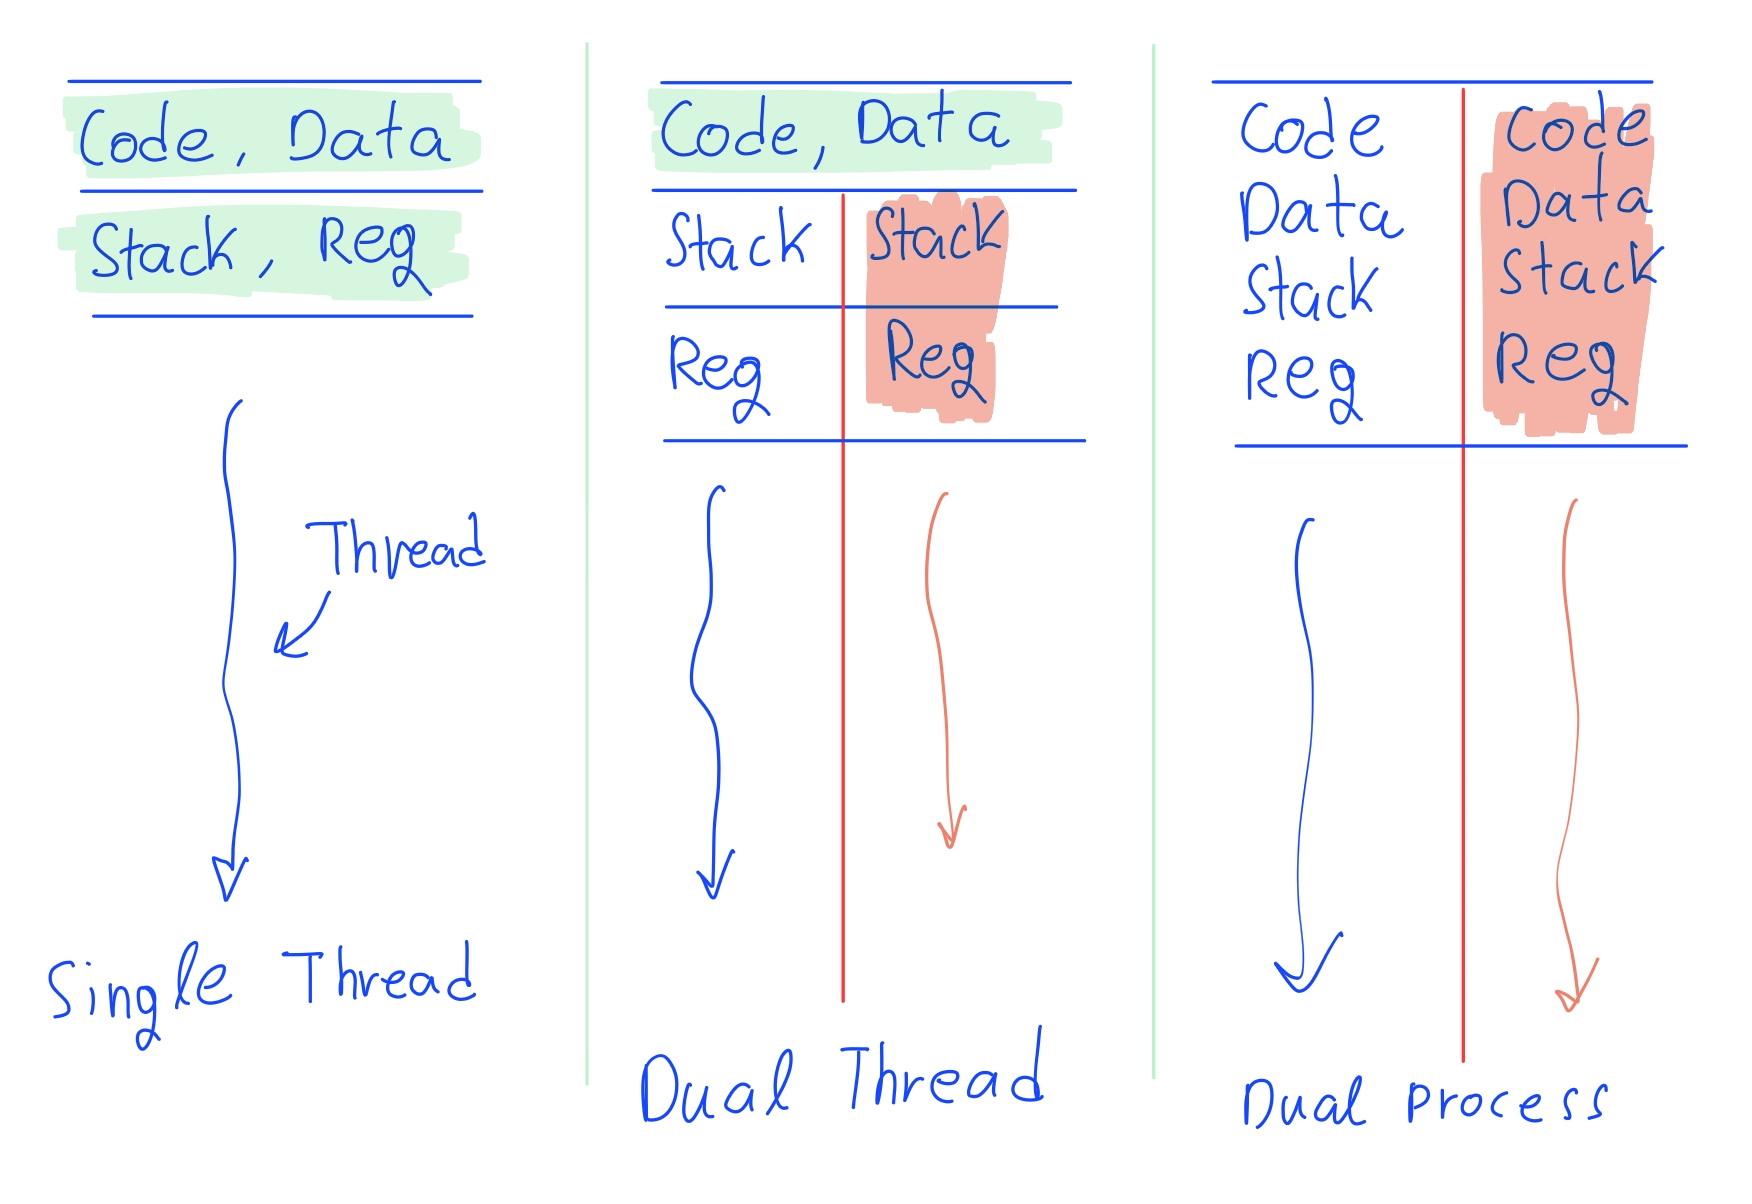
\includegraphics[width=11cm,keepaspectratio]{../media/lecture1-threads.png}
  \end{center}
\end{frame}

\section{Atomicity and race conditions}

\begin{frame}[fragile]
  \frametitle{A recipe}

  Suppose that two steps of the recipe for \textcolor{blue}{Dish I} read as
  \begin{enumerate}
    \item Put veggies in the (heated) frying pan. Wait 8 minutes. Take veggies
      out.
    \item Put meat in the (heated) frying pan. Wait 8 minutes. Take meat out.
    \end{enumerate}
    \vspace{0.6cm}
    \begin{block}{Question 1}
      \uncover<2->{Is everything alright with this recipe?}
    \end{block}
    \begin{block}{Question 2}
      \uncover<3->{What if two chefs (i.e. two threads) are working on the recipe?}
    \end{block}
\end{frame}

\begin{frame}[fragile]
  \frametitle{What is thread safety?}

  \begin{block}{Thread-safe class}
    A class (or piece of code) is \emph{thread-safe} if it behaves correctly
    when accessed from multiple threads, regardless of the scheduling or
    interleaving of the execution of those threads by the runtime environment,
    and with no additional synchronization or other coordination on the part of
    the calling code.
  \end{block}

  \vspace{1cm}
  \begin{block}{Example}
       \uncover<2->{\emph{The \textcolor{blue}{Dish I} \textbf{recipe} is not
           thread-safe.}}
  \end{block}
\end{frame}

\begin{frame}[fragile]
  \large{\textbf{Important:} There is not pre-existing notion of correctness.
    The developer decides what constitutes what is correct and what is not.}
\end{frame}

\begin{frame}[fragile]
  \frametitle{What is a race condition}

  \begin{block}{Race condition}
    A race condition occurs when the correctness of a computation depends
    on the relative timing or interleaving of multiple threads by the runtime.
  \end{block}

  \begin{itemize}
  \item[\faBook] More specific than thread-safety.
  \end{itemize}

    \begin{block}{Example}
      \uncover<2->{\emph{The correct completion of the recipes by two chefs
          depends on the timing of the usage of the frying pan. In other words,
          we have a \textcolor{red}{single} \textbf{race condition} in the
          ``2-chefs-2-dishes-kitchen'' program.}}
  \end{block}
\end{frame}

\begin{frame}[fragile]
  \frametitle{The root of all evil}

  \begin{itemize}
  \item[\faUserInjured] The sharing of \emph{mutable} state (e.g. the frying pan) may
    lead to inconsistent, incorrect behaviour.
    \begin{itemize}
    \item[\faBriefcaseMedical] Proper, careful synchronization.
    \end{itemize}
  \item[\faBook]<2-> \emph{Immutable}  (w.r.t the threads) shared state
    $\implies$ thread-safe code.
  \item[\faBook]<3-> \emph{No} shared state $\implies$ thread-safe code.
  \end{itemize}

  \begin{itemize}
  \item[\faSearch]<4-> How do we safely share mutable state?
  \end{itemize}

\end{frame}

\begin{frame}[fragile]
  \frametitle{Atomic operations}

  \begin{block}{Atomicity}
    An operation or sequence of operations on a shared state is atomic if it is
    \emph{indivisible}, meaning it cannot be interrupted or observed in an
    incomplete state.
  \end{block}

  \begin{itemize}
  \item[\faBook]<2-> Let S be an atomic operation. According to a thread B, a
    thread A has either finished S or not yet started S.
  \item[\faBook]<2-> Our race conditions are results of operations on shared
    state not being atomic.
    \begin{itemize}
    \item[\faUserInjured]<2-> Non-atomicity + interleaving $\implies$ problem!
    \end{itemize}
  \end{itemize}
\end{frame}

\begin{frame}[fragile]
  \frametitle{More on atomicity}

  \begin{itemize}
  \item[\faBook] All memory accesses in Java are atomic.
    \begin{itemize}
    \item[\faUserInjured] Except \texttt{long} and \texttt{double}! We might get
      a \emph{data race} with those.
    \end{itemize}
  \item[\faBook] In particular, things like ``\texttt{++}'' are \emph{not} atomic!
  \item[\faBook] Never assume you can mix atomic operations into a compound,
    atomic operation.
    \begin{itemize}
    \item[\faBriefcaseMedical] More synchronization!
    \end{itemize}
  \end{itemize}

  \begin{itemize}
    \item[\faBook]<2-> Useful details can be found from official \href{https://docs.oracle.com/javase/specs/jls/se10/html/jls-17.htm}{sources}.
    \end{itemize}

    \uncover<3->{
      \begin{block}{Next up}
        \begin{itemize}
        \item[\faSearch] How can we make non-atomic operations atomic?
        \end{itemize}
      \end{block}}
\end{frame}

\section{Intrinsic locks}

\begin{frame}[fragile]
  \frametitle{Intrinsic locks}

  \begin{itemize}
  \item[\faLock] This is Java’s simplest form of thread synchronization.
  \end{itemize}

  \uncover<2->{
    \begin{itemize}
    \item[\faBook] An intrinsic lock (or monitor lock) is Java’s built-in locking
      mechanism.
    \item[\faBook] Every Java object has one intrinsic lock (also called a monitor).
    \item[\faBook] One can use an object's intrinsic lock to \emph{protect} access
      to a block of code.
    \item[\faBook] A thread \textbf{must acquire} the object's lock before
      executing synchronized code.
    \item[\faBook] When the thread exits the block, the lock is automatically
      released.
    \end{itemize}}

\end{frame}

\begin{frame}[fragile]
  \frametitle{Intrinsic locks (examples)}

  \begin{lstlisting}[language = Java , frame = trBL , firstnumber = last , escapeinside={(*@}{@*)}]
    //The method's instance is the underlying monitor of the lock
    public synchronized void increment() {
      count++;
    }
  \end{lstlisting}

  \begin{lstlisting}[language = Java , frame = trBL , firstnumber = last ,
    escapeinside={(*@}{@*)}]
    //You can lock specific blocks. Observe the explicit (this).
    public void increment() {
      synchronized(this) {
        count++;
      }
    }
  \end{lstlisting}

\end{frame}

\begin{frame}[fragile]
  \frametitle{Intrinsic locks (examples)}

  \begin{lstlisting}[language = Java , frame = trBL , firstnumber = last ,
    escapeinside={(*@}{@*)}]
    //You can lock static methods to restrict ANY invocation.
    public static synchronized void log(String message) {
      System.out.println(message);
    }
  \end{lstlisting}

\end{frame}

\begin{frame}[fragile]
  \frametitle{Intrinsic locks (2)}
  \begin{block}{Locking and atomicity}
    If access to some shared state is controlled by a \textbf{sigle} lock, then
    all operations on it are perceived as atomic: a thread can't access said
    state while another thread is in the middle of an operation on it.
  \end{block}

  \begin{block}{Important}
    A shared state may consist of multiple variables. Pay attention to their
    \emph{dependence}: Synchronizing individual variables separately does not
    ensure atomicity when variables are related.
  \end{block}

  \begin{itemize}
  \item<2->[\faUserInjured] Make sure you use only \textbf{one} lock per
    ``dependent group'' of variables, for operations that must happen as a unit.
  \end{itemize}
\end{frame}

\begin{frame}[fragile]
  \frametitle{Intrinsic locks (3)}

  \begin{itemize}
  \item[\faBook]<1-> Locks ``serialize'' access to shared resource, thus making
    operations \emph{sequential}.
  \item[\faUserInjured]<1-> This means that there is performance overhead
    associated to locks.
  \item[\faBook]<1-> Make sure you use locks efficiently and protect the minimum
    amount of code.
  \end{itemize}
\end{frame}

\begin{frame}[fragile]
  \frametitle{Code Listings}

  \begin{itemize}
  \item[\faCode]<1-> CookingBenignRace: ``Two-chefs'' but correctness is
    independent of the interleaving.
  \item[\faCode]<1-> CookingRace: ``Two-chefs'' with a shared
    pan. Race condition is present.
  \item[\faCode]<1-> CookingFixed: ``Two-chefs'' with a shared pan, synchronized.
  \item[\faCode]<1-> WithdrawFixed: Synchronized check-then-withdraw example.
  \item[\faCode]<1-> Counter.java: Example from Week 8 on a shared counter.
  \item[\faCode]<1-> CounterPlus.java: Example from Week 8 on a shared counter.
  \item[\faCode]<1-> GasTankRace: Gas storage example with a nice race
    condition.
  \item[\faCode]<1-> GasTankRace: Gas storage example with a nice race condition.
  \end{itemize}
\end{frame}

\begin{frame}{}
  \centering \huge
  Thank you!
\end{frame}

\end{document}

%%% Local Variables:
%%% mode: latex
%%% TeX-engine: xetex
%%% TeX-master: t
%%% End:
